% Created 2023-11-28 Tue 13:47
% Intended LaTeX compiler: pdflatex




\documentclass[presentation, smaller]{beamer}
\usepackage[utf8]{inputenc}
\usepackage[T1]{fontenc}
\usepackage{graphicx}
\usepackage{longtable}
\usepackage{wrapfig}
\usepackage{rotating}
\usepackage[normalem]{ulem}
\usepackage{amsmath}
\usepackage{amssymb}
\usepackage{capt-of}
\usepackage{hyperref}
\usepackage{amsmath,amssymb}
\usetheme[]{default}
\usepackage{tikz}
\usetikzlibrary[topaths] \newcount\mycount
\usepackage{pgf}

\pgfmathsetseed{\number\pdfrandomseed} % to ensure that it is randomized
% use \randomseed for xelatex

\newcommand{\thecmd}[1]{%
\pgfmathsetmacro{\thenum}{int(random(ceil(#1-#1/4),floor(#1+#1/4)))}%
\thenum%
}%
\usepackage{xcolor}
\usepackage{framed}
\usepackage{amsthm}
\usepackage[utf8]{inputenc}

\colorlet{shadecolor}{CoalGray!15}

\newcommand{\propnumber}{} % initialize
\newtheorem*{prop}{Proposition \propnumber}
\newenvironment{propc}[1]
{\renewcommand{\propnumber}{#1}%
\begin{prop}}
{\end{prop}}
\frenchspacing
\usetheme{purduegold}
\author{John Biechele-Speziale, Kushagra Kapoor, Jae Heo}
\date{\today}
\title{POMDPs: Myths, Legends, and Reality}
\hypersetup{
 pdfauthor={John Biechele-Speziale, Kushagra Kapoor, Jae Heo},
 pdftitle={POMDPs: Myths, Legends, and Reality},
 pdfkeywords={},
 pdfsubject={},
 pdfcreator={Emacs 28.1 (Org mode 9.6.1)}, 
 pdflang={English}}
\begin{document}

\maketitle
\begin{frame}{Outline}
\setcounter{tocdepth}{1}
\tableofcontents
\end{frame}

\setbeamertemplate{footline}[frame number]

\section{POMDP Variants and Applications}

\begin{frame}{Model-Based Approaches: Value Iteration}
    \begin{itemize}
        \item Value Iteration for an observable discrete MDP:
        \begin{itemize}
            \item One entry per state: $V(s_1) = 0.9$
        \end{itemize}
        
        \item For a 2 state POMDP, the belief state looks like : $[0.25, 0.75]$. 
        \begin{itemize}
            \item Belief space is continuous $\implies$ No longer one entry per state.
        \end{itemize}
        \item Problem: Continuous MDP
        \begin{itemize}
            \item \textbf{key insight}: finite horizon value function is \textbf{piecewise linear and convex (PWLC)}
        \end{itemize}
        
    \end{itemize}
    
\end{frame}

\begin{frame}{Model-Based Approaches: Value Iteration}
\begin{figure}
    \centering
    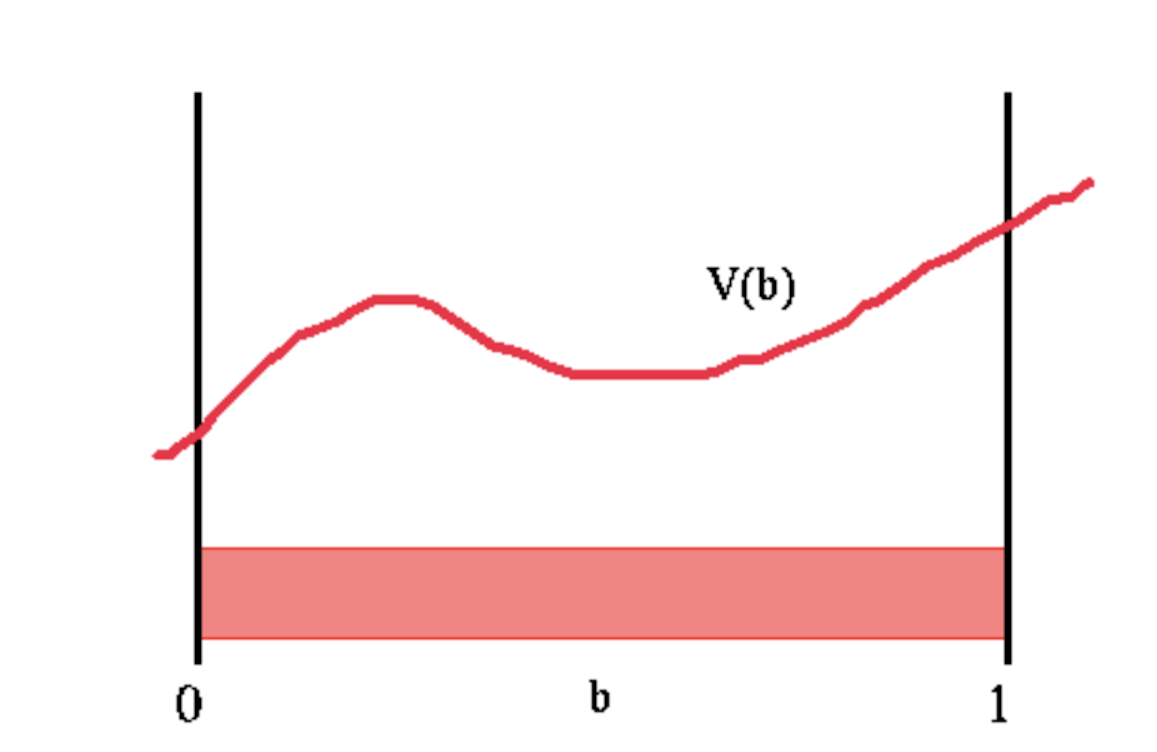
\includegraphics[scale = 0.2]{pic_1_1.png}
    \caption{Value function for a continuous belief space}
    \label{fig:enter-label}
\end{figure}
 \begin{figure}
    \centering
    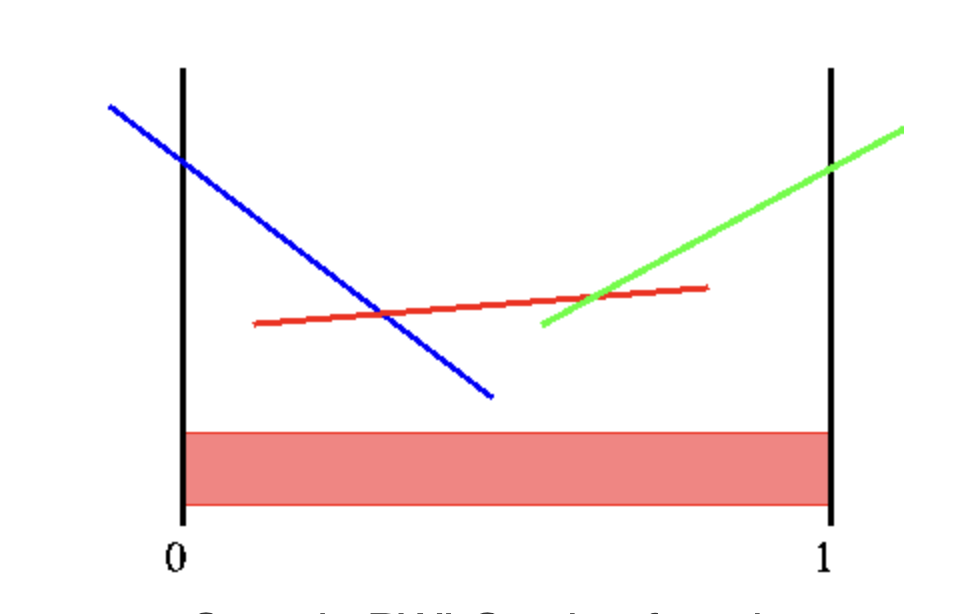
\includegraphics[scale = 0.25]{pic_2.png}
    \caption{Value function is PWLC}
    \label{fig:enter-label}
\end{figure}
\end{frame}

\begin{frame}{Model-Based Approaches: Value Iteration}
\begin{figure}
    \centering
    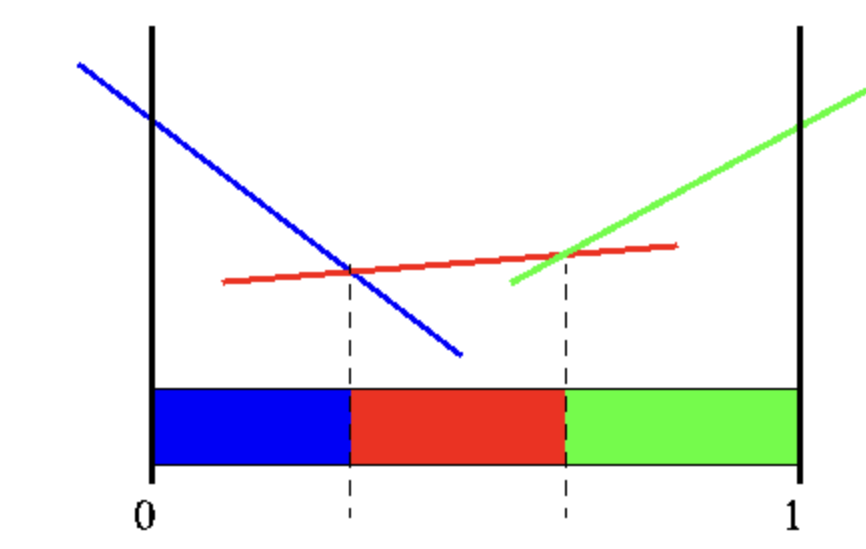
\includegraphics[scale = 0.2]{pic_3.png}
    \caption{Value function for a continuous belief space}
    \label{fig:enter-label}
\end{figure}
\begin{itemize}
    \item Big Picture: We have used properties of POMDP to simplify the problem.
    \item \textbf{Big Problem?} How to generate a finite set of points so that we can construct all of the vectors in V' (Value function for the next belief state)
\end{itemize}
\end{frame}

\begin{frame}{Model-based Approaches: Monahan’s Enumeration Algorithm (1982)}
  \textbf{Monahan’s Enumeration Algorithm:}
  \begin{itemize}
    \item Calculates all possible ways HPOMDPVn could be constructed.
    \item Exploits the known structure of the value function.
    \item Generates a finite number of vectors in each HPOMDPVn.
    \item \textbf{Exponential increase} in cardinality: $|A||Vn|^{|O|}$
    \item Regions of many generated vectors are empty and useless.
    \item \textbf{Insight:} Pruning required

  \end{itemize}

\end{frame}
\begin{frame}{Model-based Approaches: Incremental Pruning Algorithm (1996)}
  \textbf{Incremental Pruning:}
  \begin{itemize}
    \item Saves computation time by pruning dominated vectors incrementally.
    \item Recursively prunes vectors by solving a linear program. 
    \item Leads to better performance with a slow growth of constraints in the linear program.
    \item Computing exact solutions for POMDPs is \textbf{intractable, approximate solutions required.}
    
  \end{itemize}
\end{frame}

\begin{frame}{Model-based Approaches: Point-based Value Iteration Methods}
  \textbf{Approximate Solutions:}
  \begin{itemize}
    \item \textbf{Intuition: What parts of belief space are reachable? }
    \item Focuses on computing solutions for reachable parts of the belief simplex.
    \item Let the agent interact with the environment, plan over the limited set of beliefs
    \item Allows planning on a limited set of prototype beliefs, making it tractable for large state spaces.
    \item \textbf{Assumption}: updating not only value but also its gradient, the
resulting policy will generalize well and be effective for beliefs outside the set B.
  \end{itemize}
\end{frame}

\begin{frame}{Model-based Approaches: Point-based Value Iteration Methods}
  \textbf{An Example:}
  \begin{itemize}
   \item Ghasemi et. al. (2019)
   \item \textbf{key innovation}: integration of planning and perception decisions through a greedy strategy for observation selection
    \item  Avoids
combinatorial expansion of the action space
by minimizing an information-theoretic measure of
the state uncertainty.
\item involves iteratively updating a set of belief points and their corresponding alpha vectors through a process of sampling, backup, and pruning.
  \end{itemize}
  \begin{figure}
      \centering
      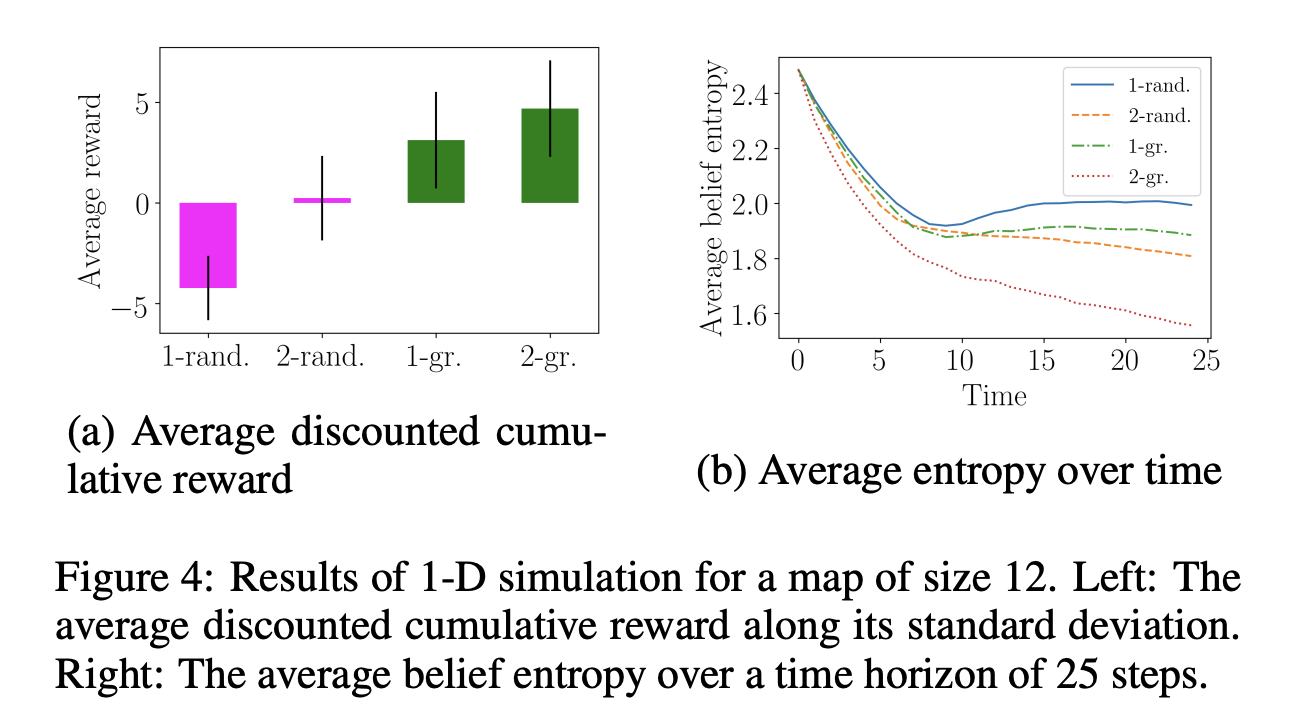
\includegraphics[scale=0.3]{mahsa.png}
      \label{fig:enter-label}
  \end{figure}
\end{frame}

\begin{frame}{Approximate Methods}
  \textbf{Grid-based Approaches:}
  \begin{itemize}
    \item Sidesteps intractability with fixed or variable grid on the belief simplex.
    \item Performs value backups, preserving only grid point values.
    \item Interpolates non-grid point values.
  \end{itemize}

  \textbf{Policy Search:}
  \begin{itemize}
    \item Searches for a good policy within a restricted class.
    \item Options include gradient ascent, stochastic local search, and methods like PEGASUS.
    \item Demonstrates success but challenging with potential local optima.
  \end{itemize}

  \textbf{Heuristic Search:}
  \begin{itemize}
    \item Builds a tree over (a,o) pairs from an initial belief node.
    \item Uses branch-and-bound for upper and lower bounds on returns.
    \item Provides an alternative approach for solving POMDPs.
  \end{itemize}
\end{frame}



\begin{frame}{Model-free Approaches}
  \textbf{Challenges Without Models:}
  \begin{itemize}
    \item When no models are available, model-based methods face challenges.
    \item QMDP requires knowledge of the complete POMDP model.
  \end{itemize}

  \textbf{Direct and Indirect Reinforcement Learning:}
  \begin{itemize}
    \item Two ways of tackling decision-making without a priori models.
    \item Direct methods map observation histories directly to actions.
    \item Indirect methods attempt to reconstruct the POMDP model by interacting with it.
  \end{itemize}
\end{frame}




\begin{frame}[label={sec:org9887ed5}]{References}
\nocite{*}
\bibliographystyle{ieeetr}
\bibliography{ref}
\end{frame}
\end{document}
